\documentclass{beamer}

\graphicspath{{img/}}

\usepackage{appendixnumberbeamer}

\usepackage{datetime}
\newdate{defensedate}{28}{07}{2017}

\usetheme[sectionpage=progressbar,subsectionpage=progressbar,numbering=fraction,
          progressbar=foot]{metropolis}

\title{Search-based Software Testing and Test Data Generation for a Dynamic Programming Language}
\subtitle{Stefan Mairhofer, Robert Feldt, Richard Torkar\\
GECCO, 2011, Dublin, Ireland.}

\date{\displaydate{defensedate}}
\author{%
  Simon Bihel\hfill\url{simon.bihel@ens-rennes.fr} \\
}
\institute{%
  COINSE Lab, KAIST, South-Korea
  % University of Rennes I \\
  % \'Ecole Normale Sup\'erieure de Rennes
}

\begin{document}

\maketitle

\begin{frame}{Table of contents}
  \setbeamertemplate{section in toc}[sections numbered]
  \tableofcontents[hideallsubsections]
\end{frame}


\section{Background}
\begin{frame}{Characteristics of dynamic languages}
  Typically:
  \begin{itemize}
    \item interpreted rather than compiled,
    \item allow runtime modification,
    \item \alert<2>{dynamically-typed},
    \item \alert<2>{complex data structures with object-oriented}.
  \end{itemize}
  \vfill{}
\end{frame}

\begin{frame}{Related Works}
  Focused on statically-typed languages.

  Complex data generation, such as strings, arrays\dots

  Object-oriented programs testing.
  \begin{itemize}
    \item Methods calls sequence.
    \item Different fitness functions, like method call distance.
  \end{itemize}
\end{frame}


\section{The Ruby Test Case Generator (RuTeG)}
\begin{frame}{Goal}
  \begin{itemize}
    \item Building an instance of the Class Under Test
    \item Set a methods call sequence with arguments
    \item Set the arguments for the final call to the Method Under Test
  \end{itemize}
  \begin{center}
    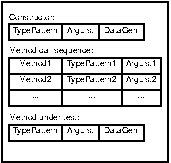
\includegraphics[height=0.5\textheight]{individual}
  \end{center}
\end{frame}

\begin{frame}{Architecture}
  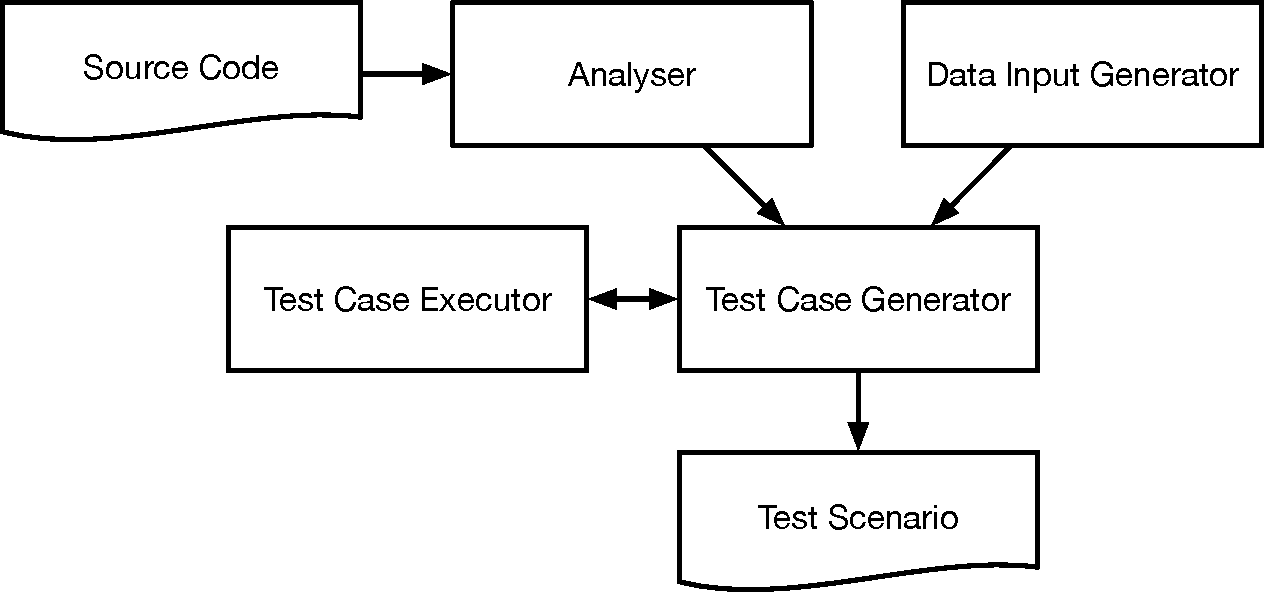
\includegraphics[width=\textwidth]{ruteg_arch}
\end{frame}

\begin{frame}{Static Analysis}
  Reduce search space.
  \begin{itemize}
    \item Method names and argument lists
    \item Methods called on arguments
  \end{itemize}

  Identify code structure and methods impacting the state of the instance.
\end{frame}

\begin{frame}{Data Input Generator}
  Basic types (numbers, strings, objects, arrays) have generators natively.

  For other types, problem-specific generators have to be \textbf{provided by the user}.
\end{frame}

\begin{frame}{Test Case generator}
  Genetic algorithm for each of the 3 parts:
  \begin{itemize}
    \item constructor;
    \item method call sequence; and
    \item method under test.
  \end{itemize}

  Fitness depending on code coverage and number of control structure lines executed.
\end{frame}


\section{Experiment}
\begin{frame}{Setup}
  Comparison with a fully random test generator (written by them).

  Fixed genetic algorithms parameters. Random initial sequence length. Tournament selection method.

  Test methods: classical code snippets as well as more complex methods from the standard library. Each test candidate was tested 30 times.
\end{frame}

\begin{frame}{Results}
  \hspace*{-1cm}%
  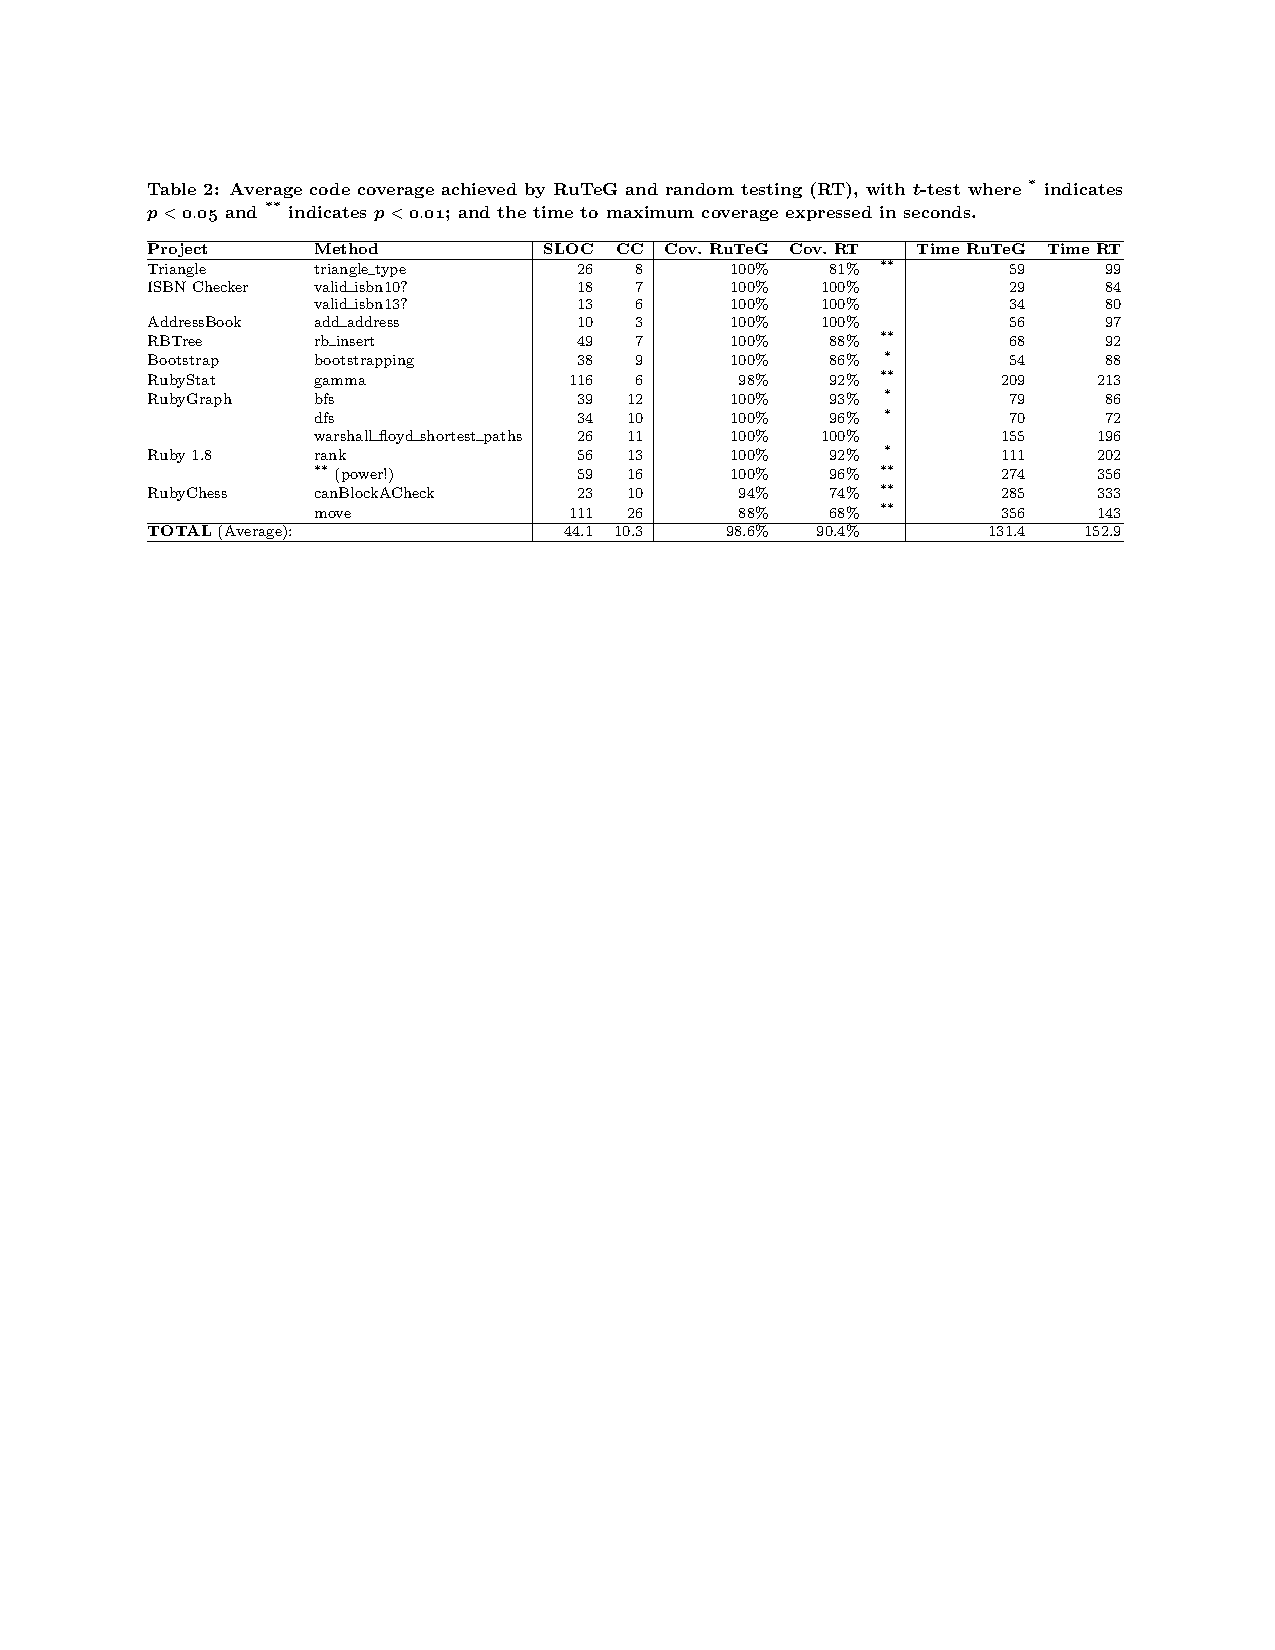
\includegraphics[width=0.99\paperwidth]{table_res}
\end{frame}

\begin{frame}{Results}
  \begin{center}
    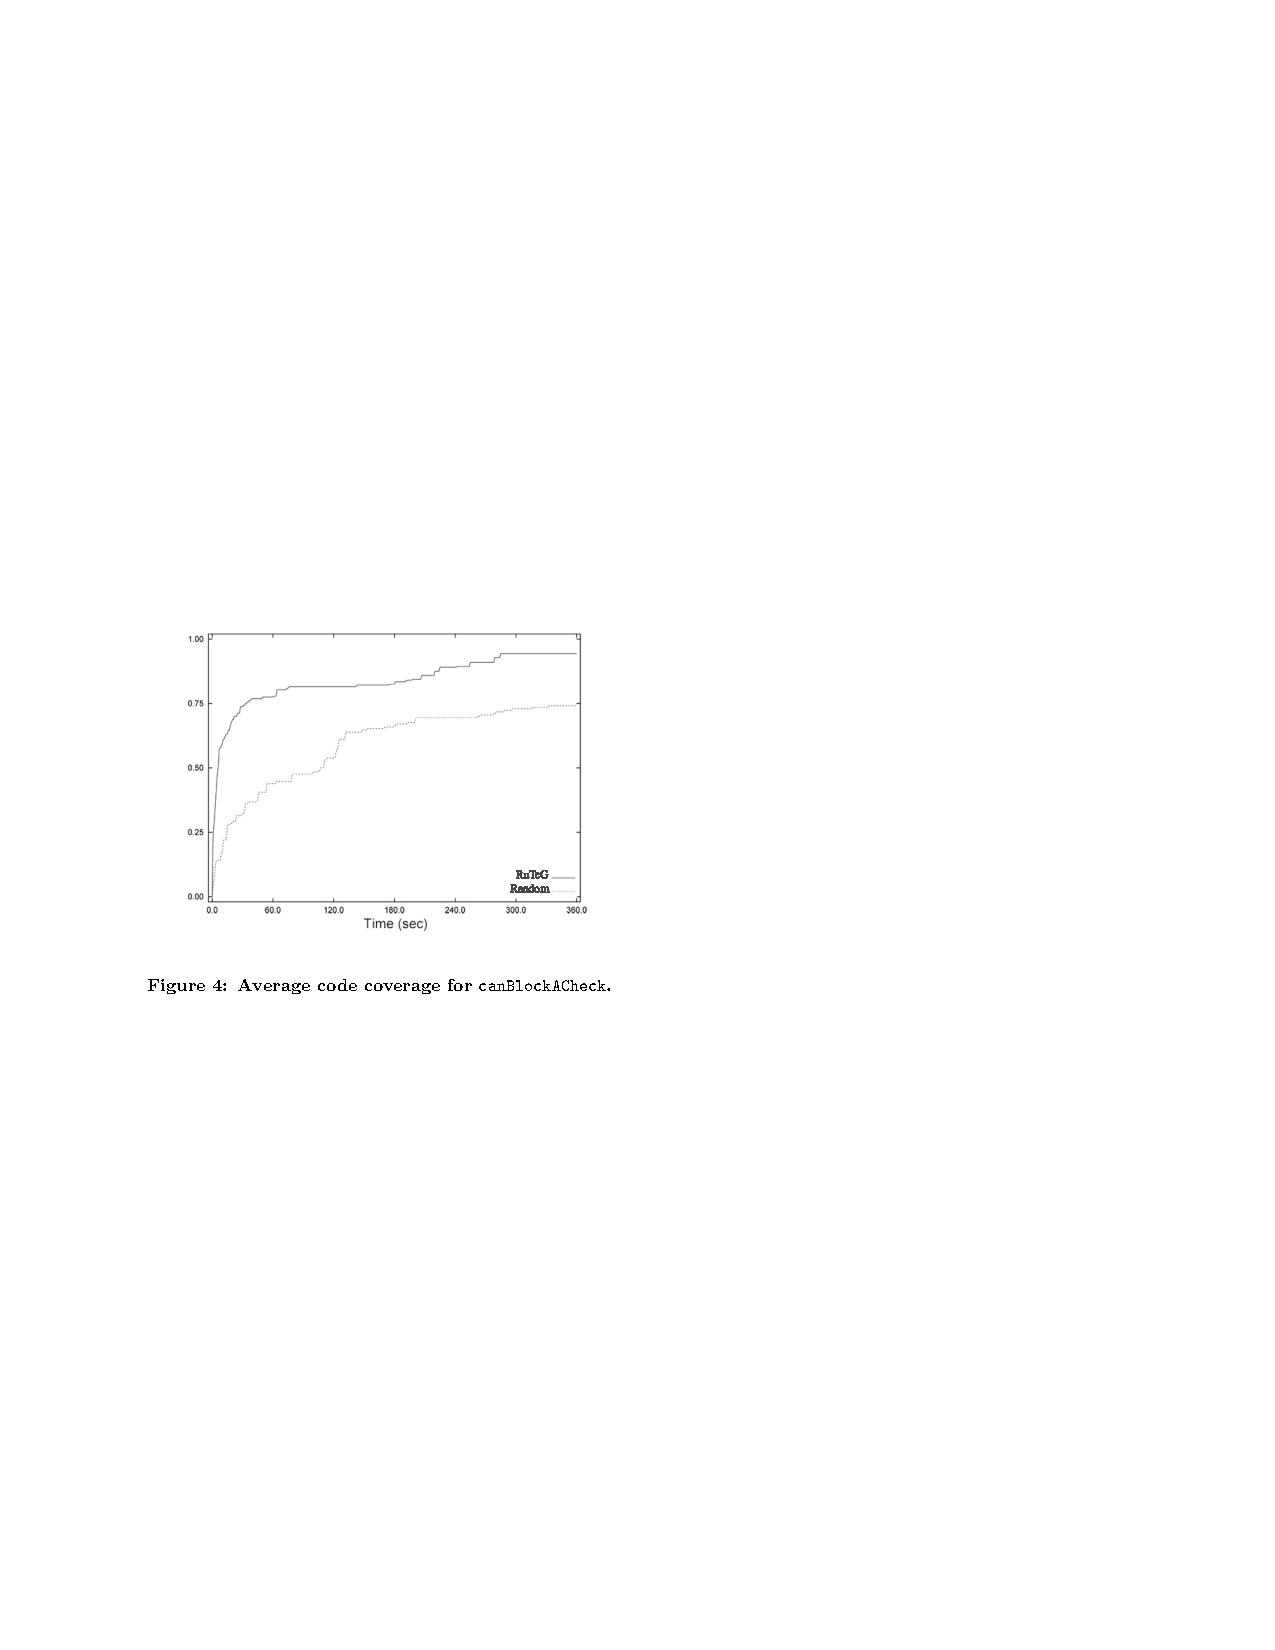
\includegraphics[width=0.9\textwidth]{ruteg_fig4}
  \end{center}
\end{frame}

\begin{frame}{Results}
  \begin{center}
    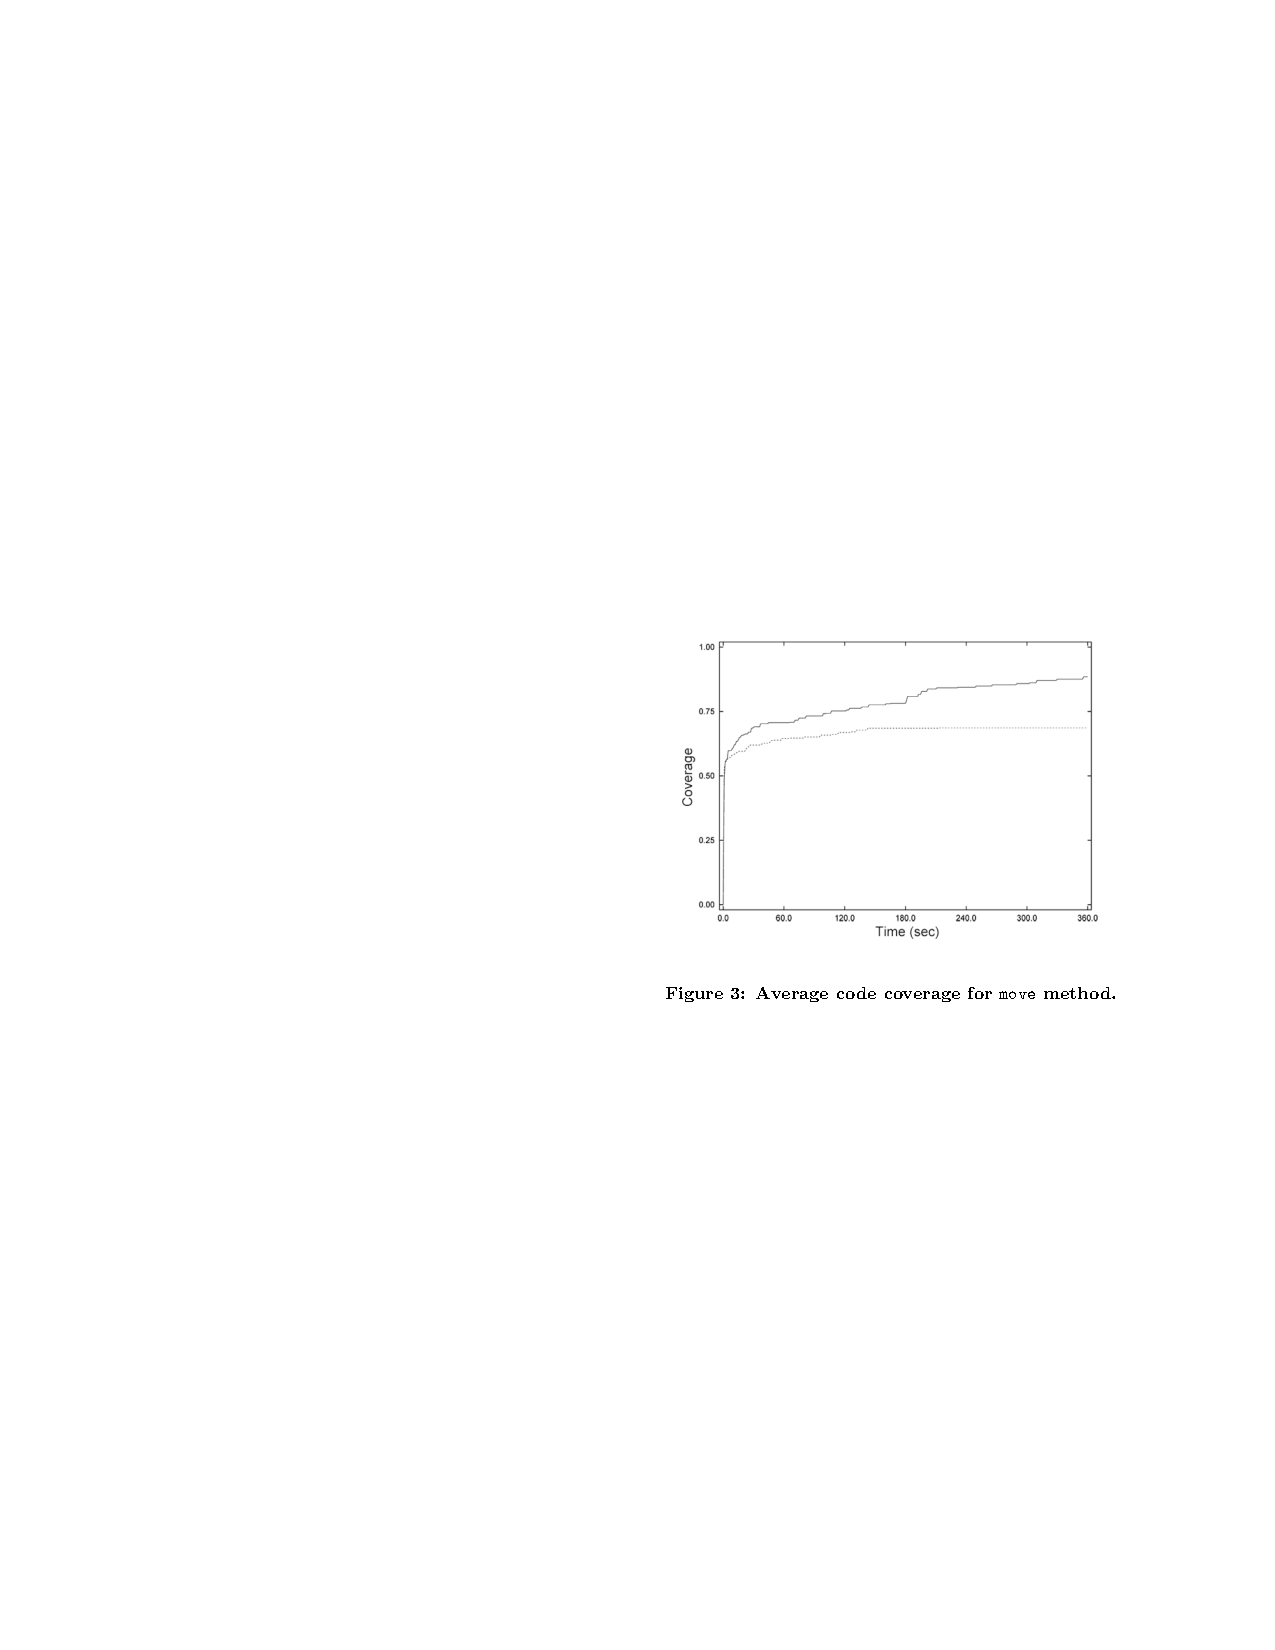
\includegraphics[width=0.9\textwidth]{ruteg_fig3}
  \end{center}
\end{frame}


\section{Discussion}
\begin{frame}{Discussion from this paper}
  \begin{itemize}
    \item Difficulty to find appropriate call sequences, especially for real life libraries.
    \item Limited by data generators.
    \item Generation of code blocks not handled.
    \item Small and complex target range values.
    \item Often times it is the state that will impact which part of the code will be executed.
  \end{itemize}
  \begin{itemize}
    \item Disqualify invalid types (but it is not clear it would work with runtime code addition).
    \item Minimal guidance on the search because of the simple fitness function.
  \end{itemize}
\end{frame}

\begin{frame}{Pros/Cons}
  Pros:
  \begin{itemize}
    \item they built something that works on some real life code; and
    \item extensive work on analysing the validity of the results.
  \end{itemize}

  Cons:
  \begin{itemize}
    \item basic experiment observations;
    \item tackling so much paradigms at once; and
    \item the paper is not very well written.
  \end{itemize}
\end{frame}

\begin{frame}{My Experience}
  No effort followed this paper.

  I tried to write a Python tool focusing only on the dynamic typing.
  It was intended for branch coverage of simple functions with primitive types and lists (containing different types and possibly other lists).
\end{frame}

\begin{frame}{What We Need To Do}
  \begin{itemize}
    \item Break down problems, focus on paradigms one at a time.
    \item Need for a fully random tester that eventually works in every situation before trying to have smarter tools.
    \item Don't underestimate technical problems and aim at generic tools.
  \end{itemize}
\end{frame}

% \section*{Conclusion}
% \begin{frame}{}
% \end{frame}

\end{document}
